\section{Additional related work}
\label{app:related}
\paragraph{Token-level speculative decoding.}
Speculative decoding~\citep{leviathan2023,chen2023} pairs a draft with a verification that keeps the target's output distribution; the draft
may be a small model or heads on the target (Medusa~\citep{medusa}, EAGLE~\citep{eagle}). A large body of
work trains the draft to raise acceptance, for example DistillSpec~\citep{distillspec} with on-policy
data and tailored divergences and domain-adapted drafts~\citep{domaindraft}. Online speculative
decoding~\citep{osd} keeps distilling a token-level draft from the queries a deployment serves; Sec.~\ref{sec:online}
does the same at the action level, where the supervision is an exact action rather than a distribution. All of it is at the token
level, where acceptance depends on matching the target's token distribution. Our setting is action-level:
only the target's decision matters, which is why we train by supervised imitation of committed actions
(Sec.~\ref{sec:train}). Our accounting of committed steps per round is the
token-level acceptance-length formula of \citet{leviathan2023} adapted to actions.

\paragraph{Action-level speculation for agents.}
Two lines exist. The first overlaps the target's \emph{decision} latency: an approximation agent runs
ahead and the target verifies. Interactive Speculative Planning~\citep{isp} and its dynamic-$k$
successor~\citep{dsp} use a cheaper prompting configuration of an API model as the approximation;
Speculative Actions~\citep{specactions} uses off-the-shelf API models and gives propositions for
single-step and asynchronous depth speculation, with latency measured on chess; Speculative Macro
Commit~\citep{smc} commits mined multi-call macros with an untrained 4B draft on three GPUs; other
systems use the same model without reasoning or off-the-shelf checkpoints~\citep{spagent,dualspec}. The second
line overlaps \emph{tool} latency: Speculative Tool Calls~\citep{stc} and PASTE~\citep{paste} execute a
predicted tool call while the model reasons, SPORK~\citep{spork} forks a probe from the running model's
own state for the same purpose, and Speculate with Memory~\citep{swm} pre-launches read-only actions from
a memory of past trajectories. AOSpec~\citep{aospec} co-speculates actions and observations so that slow
tool calls overlap generation, verifying each prediction together with the state it was made from; it
targets the regime where tools dominate, the complement of the generation-bound regime of
Sec.~\ref{sec:model}. These works bound their gain by the tool-time share (at most 2\xx{} in
\citet{stc}). LEAP reduces the number of sequential target generations and pays tool time in
full; the two compose. Speculative Actions~\citep{specactions} analyzes single-step and asynchronous
action speculation. Our framework studies synchronous proposal rounds with concurrent verification
on one shared GPU. It accounts for verification wait, segment boundaries, drafting cost and tool time
(Sec.~\ref{sec:model}). Among the self-speculation methods considered here, Speculate While You Reason~\citep{swyr},
trains the agent jointly with a self-speculation head via RL and reports Hit@1 without end-to-end
latency. LEAP studies a separately trained small action draft for a frozen target and measures wall-clock on a shared GPU.

\paragraph{Benchmarks.}
We use OpenAGI~\citep{openagi}, TaskBench~\citep{taskbench}, the $\tau^2$-bench domain of
$\tau^2$-bench~\citep{tau2bench}, and the multi-turn split of BFCL~\citep{bfcl}.

\section{Algorithm, guarantee and supervision}
\label{app:method}
\subsection{Problem, guarantee and notation}
\label{app:detail:problem}
A target agent $T$ solves a task by a sequence of actions. At step $i$ it sees a context $s_i$
(instruction, tool schemas, the actions and observations so far, and any user turns) and emits the action
$a_i = T(s_i)$, the canonical action that greedy decoding returns on $s_i$ after its reasoning; on tool benchmarks the action is
executed and its observation is appended to the context. We want to run this agent faster while every
action it executes is still its own.

Property~\ref{prop:exact} states the per-action guarantee used here.
The loop of Sec.~\ref{sec:loop} maintains this property by construction, and the harness checks it on every
task. The property holds per action, not per trajectory. The serving engine's floating-point results depend on
which requests it decodes together, and speculation verifies several contexts at once. Run alone, the target
repeats its trajectory exactly; with speculation, a small numerical difference can change a token in a long
chain of reasoning and with it a decision, after which the trajectory differs. Batching is the main source but not
the only one: with every verification decoded alone, trajectories still differ on some tasks (App.~\ref{app:success}).
Speculative Actions~\citep{specactions} calls such verification lossless; we keep the per-action guarantee and measure how
often whole trajectories differ (App.~\ref{app:success}).

\textbf{Draft and agreement.} A draft $D$ is a small model that predicts $T$'s action from the same
context, $\hat a = D(s)$, decoded greedily without reasoning. Actions are compared after
canonicalization (tool name and sorted arguments, or the reply marker for a user-facing message). On a set
of $n$ target contexts $\{(s_i, a_i)\}$ the offline \emph{agreement} of $D$ is
$\frac{1}{n}\sum_{i}\mathbbm{1}[D(s_i) = a_i]$. Its counterpart in the running system is the
per-position acceptance $q_j$ of the loop, defined in Sec.~\ref{sec:model} and compared with the offline
rate in Table~\ref{tab:agree}. Table~\ref{tab:notation} collects the notation.

\begin{table}[t]
\centering
\caption{Notation.}
\label{tab:notation}
\small
\begin{tabular}{ll}
\toprule
$T$, $D$ & target agent; draft \\
$s_i$, $a_i$ & context and target action at step $i$; $\hat a_j$: $j$-th proposal of a round \\
$k$ & proposals per round (depth) \\
$A$ & accepted proposals in a round; the round commits $A{+}1$ steps \\
$L$ & agent steps in a segment (between user turns or up to the end of the task) \\
$q_j$ & $\Pr[A \ge j]$, hit rate at position $j$; $q_1$ is the first-position acceptance \\
$c$, $e$ & committed steps per round; expected bonus-step loss at segment ends (Eq.~\ref{eq:c}) \\
$t_{\mathrm{gen}}$, $t_{\mathrm{tool}}$, $t_{\mathrm{draft}}$ & mean target generation, tool and draft-proposal times; $d = t_{\mathrm{draft}}/t_{\mathrm{gen}}$ \\
$\beta$ & round-wait inflation: mean of the slowest awaited verification over $t_{\mathrm{gen}}$ \\
$S$ & whole-task speedup, sequential over speculative wall-clock (Eq.~\ref{eq:S}) \\
\bottomrule
\end{tabular}
\end{table}

\subsection{The speculative loop}
\label{app:detail:loop}
Execution proceeds in \emph{rounds}. The draft and the target alternate; the draft never runs ahead of the
target. Given the committed prefix $s$, a round has three steps (Fig.~\ref{fig:loop}).
\begin{enumerate}
  \item \textbf{Propose.} $D$ proposes $\hat a_1,\dots,\hat a_k$ one after another, each conditioned on
  $s$ and its own earlier proposals. On tool benchmarks each proposal is executed in a copy of the
  environment so that the next proposal can see its observation; the real environment executes only
  committed actions, and an accepted proposal is not executed again: the copy in which it ran becomes the
  environment.
  \item \textbf{Verify.} $T$ generates its own action on the $k{+}1$ contexts $s$, $(s,\hat a_1)$,
  \dots, $(s,\hat a_1,\dots,\hat a_k)$, sent as concurrent requests to the same server that serves it
  alone. Let $A$ be the number of leading proposals that equal $T$'s action on their context.
  \item \textbf{Commit.} The round commits $\hat a_1,\dots,\hat a_A$ and, after them, $T$'s own action on
  the first context they do not match; if all $k$ match, that is $T$'s action on the $(k{+}1)$-st
  context, a \emph{bonus} step. The remaining verifications are discarded.
\end{enumerate}
A round thus commits $A{+}1 \le k{+}1$ steps for one target wait, and every committed action is one that
$T$ generated on the context in which it is committed (Property~\ref{prop:exact}). Rounds never cross a
\emph{segment} boundary: the end of the task, or a reply to the user, after which the next context
contains a user turn the draft cannot predict. When a proposal is a reply, no request is issued past it,
and a round that verifies the reply ends without a bonus step. $L$ denotes the number of agent steps in a
segment. Fig.~\ref{fig:timelines} shows where the time goes when every proposal is accepted and when
the first one is rejected.

\begin{proposition}[commit-eligible prefixes are teacher-forced]
\label{prop:commit}
$\hat a_j$ is committed only if $\hat a_{<j} = a_{<j}$; hence every context in which a proposal can be
committed is a prefix of the target's own trajectory, at every position $j$ of the round and not only at
$j{=}1$, and the committed action in that context is the target's teacher-forced action. Deployment
therefore draws its (context, committed action) pairs from the target's own traces; which contexts are
drawn depends on where rounds start and which proposals are accepted, a selection that
Sec.~\ref{sec:validation} measures.
\end{proposition}
\emph{Proof.} A round commits $\hat a_1,\dots,\hat a_A$ with $A = \min\{j : \hat a_j \neq a_j\} - 1$. If
$\hat a_j$ is committed then $j \le A$, so $\hat a_{<j} = a_{<j}$ and $\hat a_j$ was produced by
$D$ on $(s, a_{<j})$. Proposals made on a mismatched prefix are discarded, never committed.
\hfill$\square$

If the target's output depended only on the context, and not on the requests decoded with it or before
it, and if tool results depended only on the environment state and the call, then by
Proposition~\ref{prop:commit} and induction over rounds the committed trajectory would be exactly the
target-only one. Property~\ref{prop:exact} needs neither condition; the first does not hold exactly in our
serving engine (Sec.~\ref{sec:problem} and App.~\ref{app:success}).

\paragraph{Implementation.}
Verification responses are consumed in prefix order; as soon as context $j$ mismatches, the requests for
contexts $j{+}1,\dots,k$ are cancelled and the server aborts them, so a round never waits for a
verification it will discard. Both models are served by the same engine on one GPU; the draft is a LoRA
adapter on a 0.6B base run without reasoning (App.~\ref{app:serving}).


\begin{figure}[tbp]
\centering\setlength{\fboxsep}{2pt}
\renewcommand{\looptagnode}[1]{}\renewcommand{\looptagA}[1]{}
\resizebox{0.9\linewidth}{!}{\begin{tikzpicture}[x=1.05cm, y=1cm, font=\footnotesize]
\useasboundingbox (-1.75,-0.1) rectangle (11.4,0.78);
\foreach \x/\y/\sty/\txt in {0.2/0.45/gen/target generation, 4.0/0.45/draftbar/draft proposal, 7.8/0.45/toolbar/tool execution,
                              0.2/0.05/cancelbar/cancelled verification, 4.0/0.05/savedband/time saved, 7.8/0.05/extraband/extra time}{
  \draw[\sty] (\x,\y+0.03) rectangle (\x+0.3,\y+0.27); \node[anchor=west] at (\x+0.32,\y+0.15) {\txt};}
\end{tikzpicture}
}\par\smallskip
\begin{subfigure}{\linewidth}\centering
\resizebox{\linewidth}{!}{% (c) both proposals accepted: three steps in the time of one target step
\begin{tikzpicture}[x=1.05cm, y=1cm, font=\scriptsize, >=stealth]
\loopframe{(c) both proposals accepted}
\loopband{6.2}{10.0}{savedband}{savedline}{time saved}
\node[rowlab] at (-0.1,2.16) {sequential};
\loopbar{0}{2.4}{1.95}{gen}{0.42}{$a_1$}\loopbar{2.4}{3.2}{1.95}{toolbar}{0.42}{}
\loopbar{3.2}{6.0}{1.95}{gen}{0.42}{$a_2$}\loopbar{6.0}{7.2}{1.95}{toolbar}{0.42}{}
\loopbar{7.2}{9.4}{1.95}{gen}{0.42}{$a_3$}\loopbar{9.4}{10.0}{1.95}{toolbar}{0.42}{}
\node[rowlab] at (-0.1,0.95) {speculative};
\loopbar{0}{0.4}{1.08}{draftbar}{0.40}{$\hat a_1$}\loopbar{0.4}{1.2}{1.08}{toolbar}{0.40}{}
\loopbar{1.2}{1.6}{1.08}{draftbar}{0.40}{$\hat a_2$}\loopbar{1.6}{2.8}{1.08}{toolbar}{0.40}{}
\loopbar{2.8}{5.2}{1.13}{gen}{0.30}{verify $\hat a_1$: \checkmark}
\loopbar{2.8}{5.6}{0.78}{gen}{0.30}{verify $\hat a_2$: \checkmark}
\loopbar{2.8}{5.0}{0.43}{gen}{0.30}{bonus $a'_3$}
\draw[densely dotted, black!60] (5.6,0.38) -- (5.6,1.55);
\node[note, anchor=south west] at (5.6,1.55) {the round waits for the slowest request ($\beta$)};
\loopbar{5.6}{6.2}{1.08}{toolbar}{0.40}{}
\node[note, anchor=west] at (6.25,1.28) {commit $\hat a_1\,\hat a_2\,a'_3$: 3 steps for 1 wait};
\end{tikzpicture}
}
\caption{Both proposals accepted: three committed steps in one verification round.}
\end{subfigure}\par\smallskip
\begin{subfigure}{\linewidth}\centering
\resizebox{\linewidth}{!}{% (d) first proposal rejected: one step, plus the proposing cost
\begin{tikzpicture}[x=1.05cm, y=1cm, font=\scriptsize, >=stealth]
\loopframe{(d) first proposal rejected}
\loopband{3.2}{6.0}{extraband}{extraline}{extra time: the proposing cost $k\,(t_{\mathrm{draft}}+t_{\mathrm{tool}})$}
\node[rowlab] at (-0.1,2.16) {sequential};
\loopbar{0}{2.4}{1.95}{gen}{0.42}{$a_1$}\loopbar{2.4}{3.2}{1.95}{toolbar}{0.42}{}
\node[rowlab] at (-0.1,0.95) {speculative};
\loopbar{0}{0.4}{1.08}{draftbar}{0.40}{$\hat a_1$}\loopbar{0.4}{1.2}{1.08}{toolbar}{0.40}{}
\loopbar{1.2}{1.6}{1.08}{draftbar}{0.40}{$\hat a_2$}\loopbar{1.6}{2.8}{1.08}{toolbar}{0.40}{}
\loopbar{2.8}{5.2}{1.13}{gen}{0.30}{verify $\hat a_1$: $\times$}
\loopbar{2.8}{5.2}{0.78}{cancelbar}{0.30}{cancelled}
\loopbar{2.8}{5.2}{0.43}{cancelbar}{0.30}{cancelled}
\draw[densely dotted, black!60] (5.2,0.38) -- (5.2,1.55);
\node[note, anchor=south west] at (5.2,1.55) {the round ends at the first mismatch};
\loopbar{5.2}{6.0}{1.08}{toolbar}{0.40}{}
\node[note, anchor=west] at (6.05,1.28) {commit $a'_1$ only: 1 step};
\end{tikzpicture}
}
\caption{First proposal rejected: one committed step, plus proposing cost.}
\end{subfigure}
\caption{\textbf{Round timelines with $k=2$.} Illustrative durations. A successful round waits for the
slowest required verification; on a mismatch, unused requests are cancelled. Tool execution for
proposals occurs while proposing, and accepted environment states are adopted.}
\label{fig:timelines}
\end{figure}


\subsection{Training the draft on the target's committed actions}
\label{app:detail:train}
\textbf{Supervision.} The training set is a by-product of running the agent (Fig.~\ref{fig:loop}): every step yields a pair
$(s_i, a_i)$ of context and the target's committed action. We run $T$ once over the training tasks, log
these pairs, and fine-tune $D$ by cross-entropy on the action tokens given the context. No target logits,
no draft rollouts, and no human labels are used. The separate pass is a convenience, not a requirement:
once the speculative system runs, every action it commits is one the target generated
(Proposition~\ref{prop:commit}), whatever the draft proposed, so its commits are the same supervision.
Sec.~\ref{sec:online} trains the draft from them while the system serves.

\textbf{Predict the decision.} The label $a_i$ is the canonical action, not the target's reasoning text.
The draft is asked to reproduce a low-entropy policy's next decision, not a 32B model's output
distribution, which is what makes a 0.6B base viable. The draft runs with reasoning disabled and, on
tool benchmarks, under the tool schema as a decoding constraint. Implementation: LoRA rank 64,
$\alpha{=}128$, learning rate $3\times10^{-5}$, two to three epochs with the checkpoint chosen on a
validation split; training takes minutes on one GPU per benchmark.

\paragraph{Why imitation is a natural objective.}
By Proposition~\ref{prop:commit} (Sec.~\ref{sec:loop}), a proposal is committed only if it was generated
on the target's true prefix, so every context in which a proposal can be committed is a prefix of the
target's own trajectory, at every position and not only the first. Supervised imitation on the target's
traces trains $D$ on contexts of this kind. Acceptance depends only on the target's decision, so the label
is the canonical action, not the target's full output distribution. Plain cross-entropy on the canonical
action is therefore the natural and cheapest objective. It is a surrogate for exact-match acceptance, and
Sec.~\ref{sec:agreement} tests alternatives. The multi-step figure of merit is the per-position hit-rate
curve $q_j$ of Sec.~\ref{sec:model}, not the single-step agreement.



\section{Latency framework and additional checks}
\label{app:model}

\subsection{A latency framework for the loop}
\label{app:detail:model}

We give a latency framework for the rounds of Sec.~\ref{sec:loop}. It
separates the quantities that decide the speedup (acceptance, depth, task
structure, round cost, draft cost), and it predicts the end-to-end speedup of
a configuration from its hit rates, its draft cost and a sequential trace
(Sec.~\ref{sec:validation}), which also tests predictions using offline hit rates.

The framework covers exact-match action verification on one shared GPU. Proposing finishes
before verification begins. It does not model asynchronous draft run-ahead, semantic verification,
or mechanisms that overlap tool execution with model generation.

\paragraph{Quantities.}
For a benchmark and a target we measure the mean wall-clock of one sequential
target step $t_{\mathrm{gen}}$ (generation only), of one tool execution
$t_{\mathrm{tool}}$, and of one draft proposal $t_{\mathrm{draft}}$, and write
$d = t_{\mathrm{draft}}/t_{\mathrm{gen}}$. The \emph{hit rates}
$q_j = \Pr[A \ge j]$, $j = 1,\dots,k$, are the probabilities that the first $j$
proposals of a round all match; $q_1$ is the first-position acceptance. The
\emph{round-wait inflation} $\beta$ accounts for the round waiting for the
slowest of the $A{+}1$ verifications it uses: its generation cost is the
expected maximum of those requests rather than one mean step, written
$\beta\, t_{\mathrm{gen}}$. If the awaited step times were
independent draws from the sequential step-time distribution,
$\beta = \sum_{a} \Pr[A{=}a]\; \mathbb{E}[\max_{a+1}] / t_{\mathrm{gen}} \ge 1$, a
closed form in the empirical distribution; consecutive steps are correlated,
so we also replay the actual trace (Sec.~\ref{sec:validation}). We compare both estimates with the measured value (Fig.~\ref{fig:components}(b)).

\paragraph{Commits per round.}
A round commits $A{+}1$ steps unless the segment ends inside the accepted
prefix, in which case the bonus step is lost. Writing $e$ for the expected loss
per round,
\begin{equation}
  c \;=\; 1 + \sum_{j=1}^{k} q_j \;-\; e,
  \qquad e \;=\; \Pr[\text{segment ends within the accepted prefix}].
  \label{eq:c}
\end{equation}
If hits were independent with rate $p$ and segments were long ($e \to 0$),
Eq.~\ref{eq:c} would be the token-level expected acceptance length of
\citet{leviathan2023}, $c = 1 + p + \dots + p^{k}$. Measured hit rates decay
faster than $q_1^{\,j}$ (Fig.~\ref{fig:components}(a)), partly because rounds
reach task or user-turn boundaries. Acceptance conditional on an existing proposal and an accepted
prefix need not decline (Table~\ref{tab:agree}). On OpenAGI the second and third positions exist in
81\% and 62\% of the rounds. For the same reason $e$ is not small on short
tasks (0.38 on OpenAGI, whose tasks average 4.2 steps). In all cases
$c \le \min(k{+}1, L)$: short segments cap the achievable depth regardless of
acceptance.

\paragraph{Round time and speedup.}
Let $D$ be the mean proposing time per round, including proposal-tool execution, divided by
$t_{\mathrm{gen}}$. Let $f$ be the fraction of sequential steps that execute a tool and $g$ the
mean number of target-executed tool actions per round. Write $\tau=t_{\mathrm{tool}}/t_{\mathrm{gen}}$.
A sequential step costs $t_{\mathrm{gen}}(1+f\tau)$. A speculative round costs approximately
$t_{\mathrm{gen}}(D+\beta+g\tau)$. Accepted proposal states are adopted, so their tool costs are
included in $D$ only once. For comparable work in the two arms, the speedup is
\begin{equation}
 S\simeq\frac{c(1+f\tau)}{\beta+D+g\tau}
 \quad\xrightarrow{\;\tau\to0\;}\quad\frac{c}{\beta+D}.
 \label{eq:S}
\end{equation}
This is the same model as Eq.~\ref{eq:main:S}. If every round makes exactly $k$ proposals and
tool time is negligible, then $D=kd$. More generally, if each proposal executes a tool and
$f=g=1$, then $D=k(d+\tau)$ and the denominator is $\beta+k(d+\tau)+\tau$.

The framework separates four effects. Acceptance controls $c$ and the number of awaited
verifications. Depth can increase $c$, proposing cost and verification wait. Segment boundaries
limit both the number of proposals and the bonus action. The draft's relative cost enters through
$D$, which explains why a smaller draft can be faster at comparable acceptance
(Sec.~\ref{sec:selfspec}). With negligible tool time, two bounds follow:
$S\le c/\beta\le(k+1)/\beta$. For long segments with independent hits, the acceptance ceiling
approaches $1/((1-p)\beta)$ as $k$ grows. When all $k$ proposals are made, their cost $kd$ keeps
growing, so deeper speculation eventually stops paying off.

Verification issues up to $k+1$ target requests per round. The number of requests per committed
step is therefore at most $(k+1)/c$. Discarded requests are cancelled early; the measured completion-token
ratio is 1.16 on $\tau^2$-bench. These costs apply to our synchronous propose--verify schedule.
Speculative Actions~\citep{specactions} overlaps draft and target execution, so its latency analysis
uses a different execution schedule.

\paragraph{Interpreting acceptance.}
For long segments, independent hits of probability $p$, negligible tool time and exactly $k$
proposals per round, the model becomes
\begin{equation}
 S(p)\simeq\frac{1+p+\cdots+p^k}{\beta(p)+kd}.
 \label{eq:main:acceptance}
\end{equation}
The numerator is nonlinear for $k\ge2$, and verification wait can vary with $p$. Boundaries add
another dependence: a one-action segment commits only one action even with perfect agreement.
Thus equal acceptance need not imply equal speedup.

The measured controls in Fig.~\ref{fig:curve} have different accepted-prefix distributions,
segment truncation and proposing costs. Pooled acceptance alone does not identify those quantities,
so Eq.~\ref{eq:S} does not imply a universal speedup curve in that acceptance rate.
For example, the untrained TaskBench draft produces no usable proposal in 38\% of rounds. Those
rounds consume proposing time and commit a target action, although no proposal enters the
accepted/compared ratio. The framework therefore uses per-position rates, boundary loss and
round costs explicitly. Tables~\ref{tab:model} and~\ref{tab:four} retain the measured inputs;
the size and online studies are shown separately in Figs.~\ref{fig:size} and~\ref{fig:online}.

\paragraph{Choosing $k$.}
For negligible tool time, write $\pi_k$ for the fraction of rounds that make a $k$-th proposal.
The proposing cost is $D_k\simeq d\sum_{j\le k}\pi_j$; proposals can stop at segment boundaries.
Write $\Delta\beta_k$ for the growth of
$\beta$ from awaiting one more request. With $B_k = \beta_k + d \sum_{j \le k} \pi_j$ the round cost at
depth $k$, so that $S_k = c_k / B_k$, a $k$-th proposal pays off if and only if
\begin{equation}
 c_k-c_{k-1}>S_{k-1}(B_k-B_{k-1}).
 \label{eq:main:depth}
\end{equation}
By Eq.~\ref{eq:c}, the gain $c_k - c_{k-1}$ is $q_k$ minus the
growth of $e$, plus any change in the earlier hit rates, which move because depth changes where rounds
start. If end effects are negligible and increasing depth leaves the earlier hit rates and proposal probabilities unchanged, the condition simplifies to
\begin{equation}
  q_k \;>\; S_{k-1}\,\bigl(\pi_k\, d + \Delta\beta_k\bigr),
  \qquad\text{or, with } \pi_k = 1 \text{ and } \Delta\beta_k = 0,\qquad
  q_k \;>\; S_{k-1}\, d .
  \label{eq:k}
\end{equation}
\begin{corollary}[depth with stable earlier-position rates]
\label{cor:k}
Assume negligible end effects and unchanged earlier-position hit rates and proposal probabilities when increasing depth. Adding a $k$-th proposal pays off when its hit probability exceeds the
current speedup times the marginal cost of the proposal: the draft's relative
cost, paid only in the rounds that reach the position, plus the extra round-wait
inflation. Near the end of a segment an accepted extra proposal can replace the bonus step instead of
adding one, so on short tasks the rule overstates the value of depth. No proposal is made past the segment
end ($\pi_k = 0$ for $k > L$); when $\Delta\beta_k=0$, setting $\pi_k=1$ upper-bounds the marginal drafting cost; this need not be conservative if verification wait also increases.
\end{corollary}
Using this approximation as a depth heuristic requires offline hit rates, draft latency, and an estimate of the change in verification wait. The following examples illustrate the heuristic rather than establish reliable configuration ranking. The planning hit rates are from the $k=5$ runs; the speedups compare separate depth runs. On OpenAGI
($d = 0.06$) the simplified threshold is about $0.09$ and selects $k = 4$
($q_3 = 0.31$, $q_4 = 0.14$, $q_5 = 0.08$); with $\pi_4 = 0.41$, $\pi_5 = 0.15$
and $\Delta\beta \approx 0.015$ per position the thresholds fall to $0.06$ and
$0.04$, and the rule predicts gains of a few hundredths up to $k = 5$; the measured speedup rises from
1.34\xx{} at $k{=}1$ to 1.51\xx{} at $k{=}3$ and 1.57\xx{} at $k{=}5$ (Table~\ref{tab:model}), the last
step within the bootstrap interval. On TaskBench ($d = 0.07$, threshold about $0.10$; $q_2 = 0.37$,
$q_3 = 0.22$, $q_4 = 0.16$, $q_5 = 0.06$) it selects $k = 4$, and the measured speedup rises
from 1.27\xx{} at $k{=}1$ to 1.37\xx{} at $k{=}3$ and 1.41\xx{} at $k{=}5$
(Table~\ref{tab:model}), the last step again within noise. On BFCL (threshold $0.02$, $q_2 = 0.07$)
it selects $k = 2$, and the measured speedup is 1.15, 1.20 and 1.19\xx{} at $k = 1$, 2 and 3; on $\tau^2$-bench (threshold $0.02$, $q_2 = 0.35$, $q_3 = 0.27$) it predicts that $k = 3$ gains further,
and the measured speedup rises from 1.58\xx{} at $k{=}2$ to 1.79\xx{} at $k{=}3$
(Table~\ref{tab:model}).

\paragraph{Assumptions.}
The framework assumes that (a) both arms do the same work. Every committed action is
target-authored, but a speculative trajectory can differ from the target-only one
(App.~\ref{app:success}); per run, the speculative arm commits between 3.9\% fewer and
2.5\% more steps than the sequential arm in the configurations of Table~\ref{tab:model};
(b) concurrent verification on a dedicated GPU is close to free: on the Qwen3 target we measure
$+1$ to $+4\%$ per generated token with up to four concurrent requests and
unchanged generation length, so $\beta$ is a max-of-$n$ effect rather than a
throughput effect (on the Gemma planning configurations of Table~\ref{tab:four}, measured $\beta$
exceeds the offline-hit replay by 0.05--0.13, Sec.~\ref{sec:validation}); (c) tool time is small relative to generation on the
benchmarks we use (simulated backends, $\le 0.07$\,s per step); we exercise the
$t_{\mathrm{tool}}$ terms by adding 2 or 5\,s to every executed tool step on $\tau^2$-bench and BFCL
(Table~\ref{tab:tool}); (d) proposing and
verifying do not overlap, as in Sec.~\ref{sec:loop}; a draft that ran ahead of
the target could hide part of the proposing cost $D$, which we leave to future work; (e) the
harness cancels discarded verifications (Sec.~\ref{sec:loop}), and we report the
residual idle time separately.

\section{Complete experimental results}
\label{app:results}
\label{app:detail:experiments}
\subsection{Setup}
\label{app:detail:setup}
We use two targets. The main one is Qwen3-32B (temperature 0, reasoning enabled); the second,
Gemma-4-31B-it, repeats the whole pipeline in Sec.~\ref{sec:results4}. The drafts are
Qwen3-0.6B, 1.7B and 4B, each with a LoRA adapter trained as in Sec.~\ref{sec:train} on the traces of
one target and one benchmark; the 0.6B draft is the main one, and the offline rates in this section are
for the Qwen3 target. Target and draft are served on one H100; the draft is co-located with the target
and takes about a tenth of the GPU memory. Splits are task-disjoint.
OpenAGI~\citep{openagi}: 250 train / 63 test tasks, 1{,}090 training pairs, ReAct-style planning with a
fixed tool set. TaskBench~\citep{taskbench}: 228 train / 60 test tasks, 1{,}120 pairs, strict canonical
tool schemas; no test task's tool sequence appears in training. $\tau^2$-bench~\citep{tau2bench}: we use its telecom domain only, in solo mode (the agent works without a
simulated user); 60 / 14 / 40 train / validation / test tasks, 932 pairs, 44 tools executed against the
benchmark's local backend. BFCL is the multi-turn split of the Berkeley Function
Calling Leaderboard~\citep{bfcl}: 130 train / 60 test tasks, 1{,}254 pairs; user
turns are speculation boundaries and proposals execute in cloned environments. Each test task is run once
sequentially (target only) and once speculatively on the same node and service, and we report the pooled
ratio $\sum \text{seq} / \sum \text{spec}$ of whole-task wall-clock (App.~\ref{app:serving} gives the timing protocol).

\begin{table}[t]
\centering
\caption{\textbf{Offline action agreement with the Qwen3-32B target} (exact match on the target's own
held-out contexts; repeated predictions averaged per context, except the $\tau^2$-bench
32B-reason reference, which uses the mode of three passes). ``32B-direct'' is the target with
reasoning disabled; ``32B-reason'' is the target itself with reasoning on, replayed on the same contexts,
i.e. on the planning benchmarks its agreement with its own earlier pass, a reference set by the engine's nondeterminism rather than a bound. The three prior-work columns are an off-the-shelf small model, a cheaper
configuration of the same model, and the target as its own draft, for which ``32B-reason'' is the reference, all
measured in one setting. BFCL rows are on 99 development contexts and count every decision, a turn end or an exact tool group;
the tool-group rate used for the acceptance comparison is in Table~\ref{tab:agree}. $\tau^2$-bench labels were sampled from the target at temperature 0.6,
and all $\tau^2$-bench columns are measured against them; there, as on BFCL, the 32B-reason column replays the
target (reasoning on, temperature 0) on the same contexts.}
\label{tab:offline}
\small
\resizebox{\linewidth}{!}{%
\begin{tabular}{lrrrrr}
\toprule
 & & \multicolumn{3}{c}{drafts used in prior work} & ours \\
\cmidrule(lr){3-5}\cmidrule(lr){6-6}
benchmark & contexts & untrained 0.6B & 32B-direct & 32B-reason & trained 0.6B \\
 & & {\scriptsize\citep{smc}} & {\scriptsize\citep{isp,dsp}} & {\scriptsize\citep{spork,swyr}} & \\
\midrule
OpenAGI   & 263 & 12.8 & 76.6 & 97.3 & 75.0 \\
TaskBench & 277 & 25.0 & 84.8 & 96.9 & 75.2 \\
$\tau^2$-bench   & 226 & 8.0  & 42.5 & 65.0 & 63.7 \\
BFCL      & 99  & 2.0  & 62.6 & 91.9 & 66.7 \\
\bottomrule
\end{tabular}}
\end{table}

The standard errors in Table~\ref{tab:offline_main} use 10,000 task-level bootstrap resamples.
All contexts and repeated predictions from a task stay together; each replicate recomputes the
context-weighted agreement. The evaluated sets contain 63 OpenAGI, 57 TaskBench, 14 $\tau^2$-bench
and 10 BFCL tasks. These SEs quantify task-sampling uncertainty conditional on the evaluated models
and runs, rather than variation across training seeds.


Table~\ref{tab:offline} gives the offline agreement of the drafts used below. Its columns are the draft
families of prior work, measured here in one setting: an untrained small model, the target with reasoning
disabled (a cheaper configuration of the same model), and, as a reference for self-speculation, the target
replaying itself with reasoning on (32B-reason). Training raises the 0.6B draft from 2--25\% to 64--75\% on every benchmark. On $\tau^2$-bench, whose labels were sampled at temperature 0.6, even the target replayed at temperature 0 matches only 65.0\% of them, so the trained draft (63.7\%) is 1.3 points below the target itself, and the 1.7B and 4B drafts of Sec.~\ref{sec:training} exceed it (68.1\% and 69.5\%). The target with reasoning disabled is a strong
predictor of its own decisions on the planning benchmarks (76.6 and 84.8, at or above the trained draft)
but not on the tool benchmarks: on $\tau^2$-bench it agrees with its reasoning-on decisions on 42.5\% of
contexts, 21 points below the trained 0.6B draft, and on BFCL on 62.6\%, four points below. Where the
decision depends on reasoning over a policy and a conversation, disabling reasoning changes the decision,
and a small draft trained on the reasoning-on decisions predicts them better than the target itself does
without reasoning.

\begin{table}[t]
\centering
\caption{\textbf{From offline agreement to live acceptance} for the trained 0.6B drafts. Offline:
exact match on the target's held-out contexts (Table~\ref{tab:offline}: mean over repeated predictions; BFCL: tool-group rate). Live,
from the end-to-end runs of Table~\ref{tab:four}: $q_1$, the fraction of rounds whose first proposal is
accepted; $q_2/q_1$ and $q_3/q_2$, the ratios of successive hit rates, which also count the rounds that
stop proposing before the position; $a_2$ and $a_3$, the acceptance of the second and third proposal
among the rounds that made it and accepted the earlier ones; and the pooled per-proposal acceptance.
BFCL live rates are per tool group. A dash marks a position that does not exist: $\tau^2$-bench and BFCL run
with $k{=}2$.}
\label{tab:agree}
\small
\begin{tabular}{lrrrrrrr}
\toprule
benchmark & offline & $q_1$ & $q_2/q_1$ & $q_3/q_2$ & $a_2$ & $a_3$ & per proposal \\
\midrule
OpenAGI   & 75.0 & 0.71 & 0.63 & 0.63 & 0.81 & 0.80 & 0.75 \\
TaskBench & 75.2 & 0.66 & 0.51 & 0.53 & 0.66 & 0.73 & 0.68 \\
$\tau^2$-bench   & 63.7 & 0.64 & 0.54 & --   & 0.63 & --   & 0.64 \\
BFCL      & 49.2 & 0.38 & 0.20 & --   & 0.62 & --   & 0.53 \\
\bottomrule
\end{tabular}
\end{table}

\paragraph{From agreement to acceptance.}
Table~\ref{tab:agree} puts the offline and the live rates side by side. At the first position, live
acceptance is within four points of offline agreement on OpenAGI and $\tau^2$-bench and nine points below it on
TaskBench, where the speculative run's trajectories depart from the canonical ones on more tasks
(trajectory parity 0.86 against 0.98 on OpenAGI), so the draft is scored on contexts it has not seen in
that form. On BFCL a quarter of the rounds are hand-off probes at turn boundaries that carry no proposal,
which lowers $q_1$ below the per-group rate. The hit rates fall with position ($q_2/q_1$ is 0.51--0.63),
but not because later proposals are harder: among the rounds that make a second or third proposal and
accepted the earlier ones, the acceptance ($a_2$, $a_3$) is 0.81 and 0.80 on OpenAGI against 0.71 at the
first position, and flat on TaskBench and $\tau^2$-bench. The fall comes from rounds that run into the end of
the task, or into an invalid draft output, so that the later positions do not exist: on OpenAGI the
second and third positions exist in 81\% and 62\% of the rounds. This is why the framework of
Sec.~\ref{sec:model} carries per-position rates $q_j$, which include this truncation, rather than a
single acceptance rate.



\subsection{Speedup across four benchmarks}
\label{app:detail:results4}

\begin{table}[t]
\centering
\caption{\textbf{Whole-task end-to-end speedup of LEAP: four benchmarks, three draft sizes, two targets} (one H100
shared by target and draft; $\tau^2$-bench and BFCL execute tools; 63, 60, 40 and 60 test tasks). Each benchmark
serves its three drafts in one configuration (App.~\ref{app:serving}). Agreement is the draft's offline exact-match rate (\%) on the
target's held-out contexts (BFCL: decision level); acceptance is the share of verified proposals that were
accepted in the runs (the per-proposal rate of Table~\ref{tab:agree}); $c$ is the measured number of committed steps per round (Eq.~\ref{eq:c}); the 95\% interval is a
task-level bootstrap of the pooled ratio (10{,}000 resamples). Bold marks the fastest of the three drafts for
a benchmark and target. Task success per arm shows no systematic change (App.~\ref{app:success}).}
\label{tab:four}
\footnotesize\setlength{\tabcolsep}{4pt}\renewcommand{\arraystretch}{0.92}
\begin{tabular}{llrrrrrrrc}
\toprule
benchmark & draft & steps & $t_{\mathrm{gen}}$ (s) & $k$ & agreem. & accept. & $c$ & speedup & 95\% CI \\
\midrule
\multicolumn{10}{l}{\emph{Target Qwen3-32B}} \\
\midrule
\multirow{3}{*}{OpenAGI} & 0.6B & 4.2  & 1.1  & 3 & 75.4 & 0.75 & 2.05 & 1.50\xx{} & [1.36, 1.65] \\
                & 1.7B & 4.2  & 1.1  & 3 & 77.6 & 0.78 & 2.18 & \textbf{1.55\xx{}} & [1.43, 1.68] \\
                & 4B   & 4.2  & 1.1  & 3 & 78.7 & 0.79 & 2.26 & 1.46\xx{} & [1.30, 1.62] \\
\cmidrule(lr){2-10}
\multirow{3}{*}{TaskBench} & 0.6B & 5.0  & 1.8  & 3 & 74.7 & 0.70 & 1.94 & 1.38\xx{} & [1.24, 1.55] \\
                & 1.7B & 5.0  & 1.8  & 3 & 81.0 & 0.76 & 2.07 & \textbf{1.47\xx{}} & [1.34, 1.61] \\
                & 4B   & 5.0  & 1.8  & 3 & 80.5 & 0.75 & 2.11 & 1.36\xx{} & [1.22, 1.52] \\
\cmidrule(lr){2-10}
\multirow{3}{*}{$\tau^2$-bench} & 0.6B & 13.9 & 12.4 & 2 & 63.3 & 0.65 & 1.92 & 1.61\xx{} & [1.44, 1.79] \\
                & 1.7B & 13.9 & 12.5 & 2 & 68.1 & 0.63 & 1.88 & \textbf{1.63\xx{}} & [1.46, 1.81] \\
                & 4B   & 13.9 & 12.4 & 2 & 69.5 & 0.66 & 1.90 & 1.56\xx{} & [1.43, 1.73] \\
\cmidrule(lr){2-10}
\multirow{3}{*}{BFCL multi-turn} & 0.6B & 10.1 & 10.8 & 2 & 66.7 & 0.53 & 1.44 & 1.18\xx{} & [1.08, 1.28] \\
                & 1.7B & 10.1 & 10.8 & 2 & 72.7 & 0.59 & 1.55 & 1.28\xx{} & [1.20, 1.36] \\
                & 4B   & 10.1 & 10.8 & 2 & 79.8 & 0.65 & 1.67 & \textbf{1.34\xx{}} & [1.21, 1.48] \\
\midrule
\multicolumn{10}{l}{\emph{Target Gemma-4-31B-it}} \\
\midrule
\multirow{3}{*}{OpenAGI} & 0.6B & 4.3  & 2.1 & 3 & 79.8 & 0.78 & 2.18 & \textbf{1.55\xx{}} & [1.35, 1.79] \\
                & 1.7B & 4.3  & 2.1 & 3 & 77.3 & 0.75 & 2.08 & \textbf{1.55\xx{}} & [1.35, 1.78] \\
                & 4B   & 4.3  & 2.1 & 3 & 79.9 & 0.76 & 2.15 & 1.52\xx{} & [1.34, 1.73] \\
\cmidrule(lr){2-10}
\multirow{3}{*}{TaskBench} & 0.6B & 4.9  & 2.3 & 3 & 80.1 & 0.82 & 2.30 & 1.60\xx{} & [1.47, 1.76] \\
                & 1.7B & 4.9  & 2.3 & 3 & 84.6 & 0.83 & 2.43 & \textbf{1.68\xx{}} & [1.56, 1.82] \\
                & 4B   & 4.9  & 2.3 & 3 & 84.2 & 0.85 & 2.45 & 1.62\xx{} & [1.51, 1.75] \\
\cmidrule(lr){2-10}
\multirow{3}{*}{$\tau^2$-bench} & 0.6B & 14.7 & 4.7 & 2 & 72.8 & 0.80 & 2.27 & \textbf{1.63\xx{}} & [1.50, 1.77] \\
                & 1.7B & 14.7 & 4.7 & 2 & 76.4 & 0.79 & 2.20 & 1.55\xx{} & [1.44, 1.67] \\
                & 4B   & 14.7 & 4.7 & 2 & 77.6 & 0.80 & 2.24 & 1.55\xx{} & [1.43, 1.67] \\
\cmidrule(lr){2-10}
\multirow{3}{*}{BFCL multi-turn} & 0.6B & 10.2 & 3.3 & 2 & 63.6 & 0.50 & 1.41 & 1.10\xx{} & [1.04, 1.16] \\
                & 1.7B & 10.2 & 3.3 & 2 & 69.7 & 0.55 & 1.48 & 1.12\xx{} & [1.06, 1.18] \\
                & 4B   & 10.2 & 3.3 & 2 & 74.7 & 0.66 & 1.66 & \textbf{1.16\xx{}} & [1.09, 1.23] \\
\bottomrule
\end{tabular}
\end{table}

Table~\ref{tab:four} summarizes the four benchmarks for drafts of 0.6B, 1.7B and 4B parameters
trained with one recipe, with Qwen3-32B and with Gemma-4-31B-it as the target. The Gemma rows repeat the
whole pipeline: new sequential traces on the same task splits, the same three drafts trained with the same
recipe on those traces, and the same serving configurations (App.~\ref{app:serving} gives the two serving
details that differ).

With the smallest draft, trained for GPU-minutes on the target's own traces, LEAP speeds up whole tasks by
1.18--1.61\xx{} with Qwen3 and 1.10--1.63\xx{} with Gemma, on planning-only tasks and on tasks that execute
tools. Task success shows no systematic change: across the 28 comparisons of App.~\ref{app:success}, the
speculative arm solves more tasks in 8, fewer in 8 and as many in 12, never differing by more than three.
Every committed action is target-authored, but whole trajectories can differ from the target-only run: they
are identical on 96\% of the OpenAGI and 83\% of the TaskBench tasks, while on the tool benchmarks, whose
steps reason for 10--12\,s, most trajectories take a different decision at some step (Table~\ref{tab:parity}).
On $\tau^2$-bench 37 of the 40 tasks are still scored identically by both arms with Qwen3, and with Gemma the
two arms follow identical trajectories on 52--55 of the 60--63 planning tasks. Repeating the $\tau^2$-bench main run (the
configuration of Table~\ref{tab:model}) end to end gives 1.59\xx{} [1.44, 1.77] against 1.58\xx{}
[1.44, 1.75] in the first pass.

The model of Sec.~\ref{sec:model} explains the ordering across benchmarks and the differences between the
targets. OpenAGI has the highest acceptance and $k{=}3$, so it commits the most steps per round
($c{=}2.05$ with Qwen3), but it also pays the largest end-of-task loss ($e{=}0.38$; tasks are 4 steps
long). $\tau^2$-bench has lower acceptance but long tasks ($e{=}0.11$) and a draft that is cheap next to a
12\,s target step ($k\,t_{\mathrm{draft}}/t_{\mathrm{gen}} = 0.03$). BFCL is limited by structure: its
segments between user turns average 2.6 steps, 26\% of its rounds are width-1 hand-off probes at turn
boundaries, and its second proposal is accepted in only 7\% of rounds, so $c$ is 1.44 and the ceiling
$\min(k{+}1, L)/\beta$ is about 1.7\xx{} even for a perfect draft. Changing the target changes the step
length, and with it the weight of the draft's cost. Gemma's steps are about twice as long as Qwen3's on the
planning benchmarks (2.1 and 2.3\,s against 1.1 and 1.8\,s), which lowers the draft term at a fixed draft
cost, and its drafts agree with it more often (77--85\% against 75--81\%), so its planning speedups are
higher (1.52--1.68\xx{}). Its tool steps are shorter: 2.6 times on $\tau^2$-bench (4.7 against 12.4\,s) and
three times on BFCL (3.3 against 10.8\,s). There the draft term rises from 0.03--0.04 to 0.08--0.12 and
from 0.04--0.07 to 0.11--0.19: on $\tau^2$-bench, with acceptance flat across sizes (0.79--0.80), the
smallest draft is the fastest, and on BFCL the speedups fall to 1.10--1.16\xx{} while the turn structure
that bounds the ceiling is unchanged.

The draft size follows the same logic. With Qwen3 the 1.7B draft is faster on every benchmark
(1.28--1.63\xx{}) and the 4B draft is faster still on BFCL alone. With Gemma the three drafts tie on
OpenAGI (1.55, 1.55 and 1.52\xx{}), where the ratio of committed steps between sizes is 1.00 against a cost
ratio of 1.01; the 1.7B draft is fastest on TaskBench and the 4B draft on BFCL, as with Qwen3.
Sec.~\ref{sec:training} takes this up.

In the $\tau^2$-bench main run of Table~\ref{tab:model}, two tasks end early in the speculative arm (the
re-measurement of Table~\ref{tab:four} has no such case: 40 of 40 terminate). On one context that six
test tasks share, the target, verifying three prefixes in one batch, ran to its
2{,}048-token budget without emitting an action in two of them, while the same
context parsed in the sequential arm and in the other four tasks. We attribute this to the
target's batch-dependent decoding (App.~\ref{app:success}); the commit audit passes on both tasks. The two tasks
are kept in the pooled ratio (their speculative arm is shorter), and excluding
them gives 1.58\xx{} [1.44, 1.75] as well.

\subsection{Framework validation}
\label{app:detail:validation}\label{app:validation}

We test Eq.~\ref{eq:S} as a predictor. For each configuration we take
$c$ from the measured per-position hit rates (Eq.~\ref{eq:c}), replay the
\emph{sequential} arm's per-step generation times to obtain $\beta$ (group
consecutive steps of a segment into rounds with independent hits at rate $q_1$
and take the maximum within each group), and measure $t_{\mathrm{draft}}$. The
prediction uses no timing from the speculative arm's verifications; the hit rates and the draft time are
measured in the speculative run.
Table~\ref{tab:model}, Table~\ref{tab:tool} and Fig.~\ref{fig:pred}(a) compare it with the measured
pooled speedup for twenty-one configurations spanning acceptance $0.02$--$0.79$, depth
$k \in \{1,2,3,5\}$, normalized proposing cost $D \in [0.02, 0.74]$ and added
tool latency up to $0.46$ of a target step.


\begin{figure}[tbp]
\centering
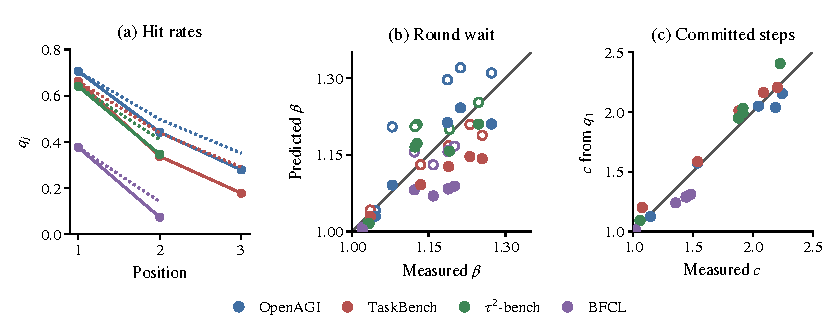
\includegraphics[width=\linewidth]{figures/fig_prediction_components.pdf}
\caption{\textbf{Component checks of the latency framework.} (a) Measured per-position hit rates (solid)
and $q_1^j$ (dotted) for the four main configurations. (b) Trace-replay $\beta$ (filled) and the
independent-step closed form (hollow), against measured values. (c) Committed steps from the
single-rate replay against measured commits. Configuration details are in Table~\ref{tab:model}.}
\label{fig:components}
\end{figure}


\begin{table}[t]
\centering
\footnotesize
\caption{\textbf{Predicted vs.\ measured speedup.} $q_j$: measured
per-position hit rates; $c$: committed steps per round; $\beta$: round-wait
inflation, predicted from the sequential arm's step times and measured from
the speculative arm; draft: the measured draft time per round divided by the
mean sequential step time (the $D$ term of Eq.~\ref{eq:S}, with rounds that
stop proposing early counted as run). ``i.i.d.''
replaces the measured hit rates by $q_j = q_1^{\,j}$. Every row was run with
cancellation, so the harness never waits on already-discarded verifications
(Sec.~\ref{sec:model}, assumption (e)) and the measured column is the speedup as run.
Rows with other $k$ exercise the depth terms of the model; Table~\ref{tab:tool} exercises its tool
terms. The 32B-direct rows use the target
itself, with reasoning disabled, as the draft; the untrained rows use the 0.6B base without an adapter.
A dash marks a position beyond the row's $k$.}
\label{tab:model}
\setlength{\tabcolsep}{3.2pt}
\resizebox{\linewidth}{!}{%
\begin{tabular}{llrrrrrrrrrrr}
\toprule
 & & & \multicolumn{3}{c}{hit rates} & & \multicolumn{2}{c}{$\beta$} & & \multicolumn{2}{c}{predicted} & \\
\cmidrule(lr){4-6}\cmidrule(lr){8-9}\cmidrule(lr){11-12}
benchmark & draft & $k$ & $q_1$ & $q_2$ & $q_3$ & $c$ & pred. & meas. & draft & i.i.d. & Eq.~\ref{eq:S} & measured \\
\midrule
OpenAGI   & trained 0.6B   & 1 & 0.74 & --   & --   & 1.54 & 1.09 & 1.08 & 0.08 & 1.35 & 1.32 & 1.34 \\
OpenAGI   & trained 0.6B   & 3 & 0.71 & 0.44 & 0.28 & 2.05 & 1.21 & 1.19 & 0.18 & 1.48 & 1.47 & 1.51 \\
OpenAGI   & trained 0.6B   & 5 & 0.70 & 0.47 & 0.31 & 2.25 & 1.24 & 1.21 & 0.22 & 1.47 & 1.54 & 1.57 \\
OpenAGI   & untrained 0.6B & 3 & 0.15 & 0.00 & 0.00 & 1.14 & 1.03 & 1.05 & 0.13 & 0.97 & 0.98 & 0.98 \\
OpenAGI   & 32B-direct     & 3 & 0.70 & 0.50 & 0.33 & 2.19 & 1.21 & 1.27 & 0.61 & 1.12 & 1.20 & 1.16 \\
\midrule
TaskBench & trained 0.6B   & 1 & 0.72 & --   & --   & 1.54 & 1.09 & 1.13 & 0.08 & 1.36 & 1.32 & 1.27 \\
TaskBench & trained 0.6B   & 3 & 0.66 & 0.34 & 0.18 & 1.88 & 1.13 & 1.19 & 0.16 & 1.56 & 1.46 & 1.37 \\
TaskBench & trained 0.6B   & 5 & 0.67 & 0.37 & 0.22 & 2.09 & 1.14 & 1.25 & 0.21 & 1.60 & 1.55 & 1.41 \\
TaskBench & untrained 0.6B & 3 & 0.21 & 0.04 & 0.00 & 1.07 & 1.03 & 1.04 & 0.07 & 1.10 & 0.98 & 0.98 \\
TaskBench & 32B-direct     & 3 & 0.74 & 0.50 & 0.33 & 2.21 & 1.15 & 1.23 & 0.73 & 1.17 & 1.17 & 1.13 \\
\midrule
$\tau^2$-bench & trained 0.6B & 2 & 0.64 & 0.35 & -- & 1.88 & 1.16 & 1.19 & 0.03 & 1.64 & 1.58 & 1.58 \\
$\tau^2$-bench & trained 0.6B & 3 & 0.71 & 0.37 & 0.27 & 2.23 & 1.21 & 1.25 & 0.04 & 1.92 & 1.78 & 1.79 \\
$\tau^2$-bench & untrained 0.6B & 2 & 0.09 & 0.00 & -- & 1.06 & 1.02 & 1.03 & 0.02 & 1.06 & 1.02 & 1.03 \\
\midrule
BFCL      & trained 0.6B   & 1 & 0.36 & --   & --   & 1.36 & 1.07 & 1.16 & 0.02 & 1.13 & 1.24 & 1.15 \\
BFCL      & trained 0.6B   & 2 & 0.38 & 0.07 & --   & 1.45 & 1.08 & 1.19 & 0.04 & 1.16 & 1.30 & 1.20 \\
BFCL      & trained 0.6B   & 3 & 0.39 & 0.07 & 0.02 & 1.48 & 1.09 & 1.20 & 0.04 & 1.16 & 1.31 & 1.19 \\
BFCL      & untrained 0.6B & 2 & 0.02 & 0.00 & --   & 1.02 & 1.00 & 1.02 & 0.05 & 0.96 & 0.97 & 0.95 \\
\bottomrule
\end{tabular}}
\end{table}

Three observations. First, the prediction is within $0.05$ of the measured
speedup for fourteen of the twenty-one configurations and within $0.10$ for all but
TaskBench at $k{=}5$ ($0.14$; harness idle time removed) and BFCL at $k{=}3$ ($0.12$).
This includes the untrained drafts on all four benchmarks (predicted $0.97$--$1.02$, measured
$0.95$--$1.03$). Second, $\beta$ replayed from sequential step times lands within
$0.07$ of the value measured in the speculative arm on fifteen configurations.
It is $0.08$ below it for the 32B-direct draft on TaskBench, $0.09$--$0.11$ below it on BFCL at
every depth without added latency and at $+2$\,s, whose step times are heavy-tailed (coefficient of
variation 1.07 against 0.3--0.5 elsewhere), and $0.11$ below it on TaskBench at $k{=}5$, where
a round issues up to six verification requests but the target server runs at most four at once
(Table~\ref{tab:serving}), so the last ones wait, which the replay does not model;
the closed form of Sec.~\ref{sec:model} is within $0.13$ on all twenty-one
(Fig.~\ref{fig:components}(b)). The largest speedup errors, TaskBench at $k{=}5$ and
BFCL, are where $\beta$ is under-predicted, which supports assumption (b) only
up to the few percent of concurrency cost the replay does not model. Third, the
i.i.d.\ shortcut $q_j = q_1^{\,j}$ is off by up to $0.18$ in $c$ in either
direction (Fig.~\ref{fig:components}(c)): it over-predicts on TaskBench and $\tau^2$-bench,
where rounds often run into the end of the task so that later positions do not
exist, and under-predicts on BFCL,
where a quarter of the rounds are hand-off probes with no proposal; the paper
therefore reports $q_j$ rather than a single acceptance rate.

\paragraph{Tool latency.}

Adding 2 or 5\,s to every executed tool step, in both arms, exercises the tool terms of Eq.~\ref{eq:S}
(Table~\ref{tab:tool}; 0.16--0.46 of a target step). The speedup falls as tools slow down: from 1.58\xx{} to
1.41\xx{} and 1.20\xx{} on $\tau^2$-bench (40 tasks), and from 1.20\xx{} to 1.07\xx{} and 1.02\xx{} on BFCL
(60 tasks). The hit rates and $c$ barely change, so the loss is in the round cost. The proposals' tools run
while proposing, which raises the draft term from 0.03 to 0.31 and 0.74 on $\tau^2$-bench and from 0.04 to
0.23 and 0.50 on BFCL, and the round pays the delay again when the target executes its own action, while the
sequential arm pays it once per step. For the four points with added latency, Eq.~\ref{eq:S} is within 0.08
of the measured speedup, and within 0.02 with the measured $\beta$; on BFCL it counts only the steps that
execute a tool and only the target's own tool steps (App.~\ref{app:predictor}). Task success, sequential against
speculative, is 22 against 22 and 22 against 27 on $\tau^2$-bench, and 34 against 34 and 34 against 33 on BFCL.

\paragraph{Prediction from offline hit rates.}
Table~\ref{tab:model} takes the hit rates from the run it decomposes. To predict a configuration before
running it, we replay the loop along the held-out sequential trajectories with the draft's teacher-forced
predictions of Table~\ref{tab:offline}: a round proposes up to $k$ actions and stops at a predicted
terminal action, the accepted prefix is the run of consecutive matches, and the round commits $A{+}1$
steps ($A$ when the prefix ends the task). Table~\ref{tab:exante} compares the replayed $q_j$ and $c$
with the live values and feeds them, with the trace-replay $\beta$ and the draft's single-stream
latency measured offline on the same held-out contexts (draft served alone, one request at a time;
0.07 of a target step on the planning benchmarks and 0.014 on $\tau^2$-bench), into Eq.~\ref{eq:S}. On OpenAGI
and $\tau^2$-bench the replay reproduces the live hit rates within 0.05 and predicts the speedup within 0.03;
on $\tau^2$-bench the hit rates come from the 14 validation tasks, sequential timing comes from the 40 test tasks, and draft latency is probed offline. On
TaskBench the replay overestimates $q_1$ (0.73 against 0.66) and the speedup (1.56 against 1.37): the
target's live trajectories depart from its sequential trace on
more tasks there (trajectory parity 0.86 against 0.98 on OpenAGI), and the draft is less accurate on the
contexts the target visits only in the live runs. An ex-ante prediction is therefore accurate to the extent that
the target is trajectory-stable under batched decoding; Proposition~\ref{prop:commit} fixes the
teacher-forced distribution only for the trajectory the target actually takes. Run on the Gemma traces
with offline draft-latency probes for 0.6B and measured per-proposal draft latency from the speculative runs for 1.7B and 4B (Table~\ref{tab:prediction_inputs}), the prediction forecasts 1.64--1.77\xx{} against 1.52--1.68\xx{} measured
on the six planning configurations, high by 0.02--0.21, and 1.60--1.62\xx{} against 1.55--1.63\xx{} on
$\tau^2$-bench, where the replay's lower hit rate on the validation tasks (0.64--0.72 against 0.76--0.77
live) offsets the same $\beta$ gap. That gap is the residual on the planning benchmarks: the trace replay
gives 1.16--1.23 where the measured round-wait inflation is 1.23--1.31. It underestimates
verification wait by 0.05--0.13 across these configurations. This gap does not identify a uniform
per-request slowdown, because the awaited contexts and generation lengths can also change.
For Qwen3 the difference is $-0.03$ to $+0.11$ across Table~\ref{tab:model}; the underlying cause
of the Gemma gap is not established.

\begin{table}[t]
\centering
\caption{\textbf{Ex-ante inputs from teacher-forced predictions.} Hit rates and committed steps per
round from replaying the loop on the held-out sequential trajectories with the offline predictions of
Table~\ref{tab:offline} (``replay''), against the live values of the runs of Table~\ref{tab:model}; the
ex-ante speedup uses the replayed values with the trace-replay $\beta$ and the draft's single-stream
latency measured offline on the held-out contexts. $\tau^2$-bench obtains hit rates from the 14 validation tasks and sequential timing from the 40 test tasks. BFCL is omitted: its
rounds are bounded by user turns with a terminal probe, which the replay does not reproduce. A dash marks
a position beyond $k{=}2$.}
\label{tab:exante}
\small
\begin{tabular}{lrrrrrrrrrr}
\toprule
 & \multicolumn{4}{c}{replay, before the run} & \multicolumn{4}{c}{live, in the run} & \multicolumn{2}{c}{speedup} \\
\cmidrule(lr){2-5}\cmidrule(lr){6-9}\cmidrule(lr){10-11}
benchmark & $q_1$ & $q_2$ & $q_3$ & $c$ & $q_1$ & $q_2$ & $q_3$ & $c$ & ex-ante & measured \\
\midrule
OpenAGI        & 0.70 & 0.45 & 0.26 & 2.03 & 0.71 & 0.44 & 0.28 & 2.05 & 1.48\xx{} & 1.51\xx{} \\
TaskBench      & 0.73 & 0.42 & 0.24 & 2.04 & 0.66 & 0.34 & 0.18 & 1.88 & 1.56\xx{} & 1.37\xx{} \\
$\tau^2$-bench & 0.59 & 0.34 & --   & 1.85 & 0.64 & 0.35 & --   & 1.88 & 1.59\xx{} & 1.58\xx{} \\
\bottomrule
\end{tabular}
\end{table}

\paragraph{Segment truncation.}
Appendix~\ref{app:length} buckets the tasks of the main runs by length. The truncation loss $e$ of
Eq.~\ref{eq:c} falls with task length as the equation says (from 0.52 to 0.30 on OpenAGI, from 0.20 to 0.07
on $\tau^2$-bench). The per-bucket speedup does not fall with it, because the draft is most often right on the
short tasks; a prediction that ignores this correlation misses by up to 0.4 in the extreme buckets, while
the run-level prediction is within 0.10.

\paragraph{Self-speculation loses on cost, not on acceptance.}
\label{app:selfspec}
The 32B-direct rows use the target with reasoning disabled as its own draft,
issued as separate requests to the same server: the self-drafting idea
of~\citet{spork,swyr} without the prefix forking and cache sharing of those systems.
Its acceptance is at least as high as the trained 0.6B draft's (0.78 vs.\
0.75 on OpenAGI, 0.79 vs.\ 0.68 on TaskBench) and it commits more steps per
round, yet its speedup is 1.16\xx{} and 1.13\xx{}: each proposal costs
$3.3$--$4.0\times$ as much wall-clock time, which raises the draft term of
Eq.~\ref{eq:S} from $0.16$--$0.18$ to $0.61$--$0.73$, and sharing the target's
server raises $\beta$ (1.19$\to$1.27 on OpenAGI). The trained 0.6B draft
reaches comparable acceptance at about a quarter of the drafting cost. On the
tool benchmarks the reasoning-free target is not even the better predictor: its
offline agreement with the target's reasoning-on decisions is 42.5\% on $\tau^2$-bench
and 62.6\% on BFCL, against 63.7\% and 66.7\% for the trained draft
(Table~\ref{tab:offline}), so self-speculation would lose there on both terms
of Eq.~\ref{eq:S}. The margin narrows with the target's step length, as the draft term predicts: on the
Gemma target of Table~\ref{tab:four}, whose planning steps are twice as long, a self-proposal costs
0.12--0.18 of a step, and self-speculation reaches 1.48\xx{} [1.23, 1.75] on OpenAGI and 1.54\xx{}
[1.46, 1.64] on TaskBench at acceptance 0.90--0.91 (draft term 0.23--0.47), against 1.55\xx{} and
1.60--1.68\xx{} for the trained drafts at a draft term of 0.09--0.23.

\paragraph{What it costs.}
Speculation trades target compute for latency. On $\tau^2$-bench the speculative arm issued 789 target requests
against 559 sequential steps and generated 1.16\xx{} the completion tokens as returned to the client
(a cancelled verification counts the tokens generated up to the cancel; the server aborts it on
disconnect); the draft adds about a tenth of the GPU memory and 3\% of the round time. The trade is
favourable when per-request latency is the constraint (interactive use, evaluation and RL rollouts) and
unfavourable for throughput-bound serving.

\begin{table}[tbp]
\centering\small
\caption{\textbf{Predictions using offline hit rates, both targets.} The eighteen size-study points
in Fig.~\ref{fig:pred}(b), using each draft's offline predictions and the original trace-replay $\beta$.
Serving configurations and measured speedups match Table~\ref{tab:main_results}. Draft timing is
either an offline single-stream probe or measured per-proposal latency from the speculative run
(``run''); the latter rows are conditional on that cost. Sequential timing is from the test trajectories;
$\tau^2$-bench hit rates are from validation trajectories. The last two columns give the trace-replay
and measured $\beta$ plotted in Fig.~\ref{fig:pred}(c).}
\label{tab:prediction_inputs}
\begin{tabular}{lllcrrrr}
\toprule
Target & Benchmark & Draft & Draft timing & Predicted & Measured & $\beta$ replay & $\beta$ meas. \\
\midrule
Qwen3 & OpenAGI & 0.6B & probe & 1.48 & 1.50 & 1.22 & 1.19 \\
Qwen3 & OpenAGI & 1.7B & run & 1.53 & 1.55 & 1.22 & 1.21 \\
Qwen3 & OpenAGI & 4B & run & 1.47 & 1.46 & 1.24 & 1.25 \\
Qwen3 & TaskBench & 0.6B & probe & 1.53 & 1.38 & 1.14 & 1.22 \\
Qwen3 & TaskBench & 1.7B & run & 1.58 & 1.47 & 1.16 & 1.21 \\
Qwen3 & TaskBench & 4B & run & 1.53 & 1.36 & 1.16 & 1.26 \\
Qwen3 & $\tau^2$-bench & 0.6B & probe & 1.58 & 1.61 & 1.14 & 1.15 \\
Qwen3 & $\tau^2$-bench & 1.7B & probe & 1.64 & 1.63 & 1.15 & 1.17 \\
Qwen3 & $\tau^2$-bench & 4B & probe & 1.62 & 1.56 & 1.16 & 1.16 \\
Gemma & OpenAGI & 0.6B & probe & 1.77 & 1.55 & 1.18 & 1.31 \\
Gemma & OpenAGI & 1.7B & run & 1.66 & 1.55 & 1.16 & 1.23 \\
Gemma & OpenAGI & 4B & run & 1.68 & 1.52 & 1.17 & 1.26 \\
Gemma & TaskBench & 0.6B & probe & 1.68 & 1.60 & 1.20 & 1.29 \\
Gemma & TaskBench & 1.7B & run & 1.74 & 1.68 & 1.23 & 1.28 \\
Gemma & TaskBench & 4B & run & 1.64 & 1.62 & 1.23 & 1.28 \\
Gemma & $\tau^2$-bench & 0.6B & probe & 1.62 & 1.63 & 1.21 & 1.34 \\
Gemma & $\tau^2$-bench & 1.7B & run & 1.61 & 1.55 & 1.25 & 1.34 \\
Gemma & $\tau^2$-bench & 4B & run & 1.60 & 1.55 & 1.24 & 1.35 \\
\bottomrule
\end{tabular}
\end{table}


\section{Additional training studies}
\label{app:training}
\subsection{Training the draft: recipe, data, input and size}
\label{app:detail:training}
The main results use one recipe per benchmark (Sec.~\ref{sec:train}). This section varies the recipe
on OpenAGI, where the held-out test set (63 tasks, 263 contexts, scored three times each at temperature
0) is cheap to re-score offline, and then varies the draft size across benchmarks. We split the OpenAGI
test tasks into \emph{seen} (40 tasks whose committed action sequence also occurs in a training task) and
\emph{unseen} (the other 23), because the two respond differently to every knob below.

\begin{table}[t]
\centering
\caption{OpenAGI offline agreement (\%) of 0.6B drafts under recipe variations. Rows marked ``ep\,7''
train for 12 epochs and pick the checkpoint by validation exact match; the Table~\ref{tab:offline} draft
trains for 3 epochs and picks by validation loss (epoch 2). Seen/unseen as defined in the text.}
\label{tab:recipe}
\small
\begin{tabular}{lrrr}
\toprule
draft & overall & seen & unseen \\
\midrule
untrained 0.6B & 12.8 & 11.5 & 14.8 \\
LoRA $r{=}64$, 3 epochs, epoch 2 by validation loss (Table~\ref{tab:offline}) & 75.0 & 82.2 & 64.5 \\
LoRA $r{=}64$, ep\,7 by validation exact match & \textbf{77.1} & \textbf{86.4} & 63.2 \\
LoRA $r{=}64$, epoch 12 & 74.1 & 83.4 & 60.4 \\
full fine-tuning, ep\,7 & 75.2 & 84.7 & 61.0 \\
LoRA $r{=}64$, ep\,7, 50\% of the pairs (535) & 72.0 & 80.5 & 59.4 \\
LoRA $r{=}64$, ep\,7, 25\% of the pairs (270) & 71.5 & 74.7 & \textbf{66.7} \\
\midrule
32B-direct (target, reasoning off) & 76.6 & 76.6 & 76.4 \\
target self-consistency & 97.3 & 98.1 & 96.2 \\
\bottomrule
\end{tabular}
\end{table}

\paragraph{Epochs, capacity and data.}
Table~\ref{tab:recipe} gives the offline agreement. Three findings. (i)~Training longer raises agreement
on seen sequences only: from epoch 2 to epoch 7 the seen score rises from 82.2 to 86.4 while the unseen
score falls from 64.5 to 63.2, and epoch 12 loses on both. (ii)~Full fine-tuning of the 0.6B model does
not beat the rank-64 adapter (75.2 against 77.1). (iii)~Halving or quartering the training pairs lowers
the overall score by five to six points, almost entirely on seen tasks; the unseen score is not monotone in the
amount of data. The two untrained references are flat across the split (32B-direct 76.6/76.4, target
self-consistency 98.1/96.2), so the seen/unseen gap is a property of the trained draft: most of what more
epochs and more data buy is familiarity with training sequences, and the unseen level of 63--67 is not
moved by these knobs. End to end the difference is small. At $k{=}3$ the epoch-7 draft reaches
1.476\xx{} against 1.455\xx{} for the epoch-2 draft, and an independent repeat of the epoch-2 run gave
1.477\xx{}; the live acceptance splits the same way (epoch 2: 82.5\% on seen and 67.0\% on unseen
tasks, 1.53\xx{} and 1.35\xx{}; epoch 7: 86.5\% and 65.0\%, 1.63\xx{} and 1.28\xx{}).

\paragraph{Draft input.}
The draft sees the task and the committed actions. Adding the target's reasoning text for the committed
steps to the draft's input raises the unseen score by at most 2.5 points (64.5 to 67.0, with the epoch-4
checkpoint) at equal overall agreement. In the live runs, however, the draft proposes positions $2..k$ before the
target has produced the reasoning for its own proposals, so training must drop the trailing one or two
thoughts; with that dropout the unseen score falls to 58--60. We therefore keep the action-only input.

\paragraph{Transfer across benchmarks.}
A trained draft is specific to its benchmark (Table~\ref{tab:transfer} in App.~\ref{app:transfer}). On each
of the other three benchmarks, the four trained drafts agree with the target about as often as the untrained
base does, within about four points. The only exception is between the two planning benchmarks: the TaskBench
draft reaches 23.3\% on OpenAGI and the OpenAGI draft 29.6\% on TaskBench, against 13.3\% and 25.3\% for the
base. This is still far below the 75\% of a draft trained on the benchmark itself. Each workload therefore
needs its own draft; training one takes minutes.

\paragraph{Draft size.}
The three drafts of Table~\ref{tab:four} bound the size axis: 0.6B is the smallest base we train and 4B the
largest that shares one H100 with the 32B target at the benchmarks' context lengths. Table~\ref{tab:size} and
Fig.~\ref{fig:size} show what varies. Offline agreement mostly rises with size
(0.6B to 4B: 75.4 to 78.7 on OpenAGI, 74.7 to 80.5 on TaskBench, where 1.7B already reaches 81.0, 63.3 to 69.5 on
$\tau^2$-bench, 66.7 to 79.8 on BFCL), and the draft's cost always does: its per-round term $D$ (Eq.~\ref{eq:S}) grows from 0.16--0.17 to
0.28--0.29 on the planning benchmarks and from 0.03--0.04 to 0.04--0.07 on the tool benchmarks, and sharing
the GPU with the 4B draft raises $\beta$ by up to 0.06. The speedup is the balance of the two. On OpenAGI and
TaskBench, where a target step takes 1--2\,s, 1.7B is the fastest draft (1.55 and 1.47\xx{} against 1.50 and
1.38\xx{} for 0.6B) and 4B falls back to the 0.6B level (1.46 and 1.36\xx{}) although it agrees most; two
independent runs of every cell give the same ordering, and Eq.~\ref{eq:S} predicts it from the sequential
trace (1.48, 1.53, 1.47 on OpenAGI; 1.53, 1.58, 1.53 on TaskBench), with TaskBench
overpredicted by 0.11--0.17. These predictions replay each draft's offline hits using the inputs in
Table~\ref{tab:prediction_inputs}; TaskBench's replayed $\beta$ is 0.05--0.10 below the measured one.
On $\tau^2$-bench, where a target step takes 12\,s and $D$ is 0.03, predicted speedups are 1.58,
1.64 and 1.62; the three drafts measure 1.61, 1.63 and 1.56\xx{}, within one another's bootstrap intervals,
with the 4B draft's calls 1.55\xx{} as long as the 0.6B draft's. On BFCL, where the 0.6B draft agrees least
and a target step takes 11\,s, every size step pays: 1.18, 1.28 and 1.34\xx{} for agreement 66.7, 72.7 and
79.8. The bootstrap intervals of neighbouring cells overlap (OpenAGI 1.7B [1.43, 1.68] against 4B [1.30,
1.62]; BFCL 1.7B [1.20, 1.36] against 4B [1.21, 1.48]), so the ordering rests on its consistency across
runs and benchmarks and on the model rather than on any single pair.

A larger draft pays exactly when its extra agreement outweighs its extra cost, and Eq.~\ref{eq:S} says
where that is: with $c$ the committed steps per round and $\beta + D$ the round cost, draft $B$ beats draft
$A$ when $c_B/c_A > (\beta_B + D_B)/(\beta_A + D_A)$. With the measured values, 4B against 0.6B has a cost
ratio of 1.12 on both planning benchmarks against a gain in $c$ of 1.09--1.10, and on BFCL a cost ratio of
1.03 against a gain of 1.16; on $\tau^2$-bench both ratios are within 0.02 of one, and the three speedups are equal
within noise. The best size therefore depends on the target step. With 1--2\,s steps a mid-size draft is
fastest; with 10--12\,s steps the draft's cost weighs little, and the larger drafts are faster on BFCL and
within noise on $\tau^2$-bench. Training cost grows with size (Table~\ref{tab:size}). The 0.6B draft, trained in
about a minute on OpenAGI, is within 0.1\xx{} of the fastest size in seven of the eight benchmark--target
pairs of Table~\ref{tab:four}, which is why it is our default and the draft of the model validation
(Sec.~\ref{sec:validation}).
For practitioners, we recommend starting with a trained 0.6B draft and $k{=}1$.



\begin{table}[t]
\centering
\caption{\textbf{Draft size.} Three drafts trained with the same recipe. Offline agreement (\%) on the
held-out contexts of Table~\ref{tab:offline}; the measured per-round draft term $D$ of Eq.~\ref{eq:S} in the
common serving configurations of Table~\ref{tab:four}; the speedup Eq.~\ref{eq:S} predicts from the
sequential trace and each draft's own offline hit predictions, with the draft timing sources
listed in Table~\ref{tab:prediction_inputs}. BFCL has no offline-hit prediction (Fig.~\ref{fig:size}).
Measured speedups are in Table~\ref{tab:four}.}
\label{tab:size}
\footnotesize\setlength{\tabcolsep}{3pt}
\resizebox{\linewidth}{!}{%
\resizebox{\linewidth}{!}{%
\begin{tabular}{lrrrrrrrrrrr}
\toprule
 & \multicolumn{4}{c}{offline agreement} & \multicolumn{4}{c}{draft term $D$} & \multicolumn{3}{c}{predicted speedup} \\
\cmidrule(lr){2-5}\cmidrule(lr){6-9}\cmidrule(lr){10-12}
draft & OpenAGI & TaskBench & $\tau^2$-bench & BFCL & OpenAGI & TaskBench & $\tau^2$-bench & BFCL & OpenAGI & TaskBench & $\tau^2$-bench \\
\midrule
0.6B & 75.4 & 74.7 & 63.3 & 66.7 & 0.17 & 0.16 & 0.03 & 0.04 & 1.48\xx{} & 1.53\xx{} & 1.58\xx{} \\
1.7B & 77.6 & \textbf{81.0} & 68.1 & 72.7 & 0.20 & 0.19 & 0.03 & 0.04 & \textbf{1.53\xx{}} & \textbf{1.58\xx{}} & \textbf{1.64\xx{}} \\
4B   & \textbf{78.7} & 80.5 & \textbf{69.5} & \textbf{79.8} & 0.28 & 0.29 & 0.04 & 0.07 & 1.47\xx{} & 1.53\xx{} & 1.62\xx{} \\
\bottomrule
\end{tabular}}}
\end{table}

\paragraph{Objective.}
Sec.~\ref{sec:train} argues that cross-entropy on the target's committed actions is a natural
objective. Table~\ref{tab:objective} lists the comparison that tests alternatives on the two benchmarks with
ground truth, TaskBench and BFCL: supervision from gold labels instead of the target's actions (does the
draft need to imitate the target rather than be correct?) and reinforcement learning from the exact-match
reward starting from the SFT draft. Offline agreement is measured for every variant; the end-to-end speedup
only where the offline gain over SFT exceeds three points; no variant reaches it. On BFCL the gold-label draft is trained with the
same recipe on the benchmark's ground-truth calls replayed in the real environment, one call per decision
(130 tasks, 1{,}200 pairs, 39\% of them turn ends; the target's traces give 1{,}254 pairs, 37\% turn ends).
It reaches 50.5\% decision agreement against 66.7\%: on the 63 held-out decisions where the target calls
a tool it ends the turn 26 times and matches the target's tool group 14 times (22\%), against 3 and
31 (49\%) for the draft trained on the target's own actions; on the 51 single-call decisions alone it matches
14 against 29. Correctness by the benchmark's standard and agreement with the target are different
objectives. The comparison changes the source of the training data, not only its labels: the gold contexts
follow the gold calls, and on BFCL the gold data has one call per decision where the target groups calls.
On TaskBench the gold-label draft reaches 69.9\% against 75.2\%. The gap is smaller there because
the annotated tool sequences often coincide with the target's: they are identical on 61 of the 228 training
tasks and use the same tools, with other argument strings, on 108 more. Reinforcement learning from the exact-match reward, run with GRPO from the SFT draft on the same
1{,}011 training contexts (eight samples per context, reward 1 for the target's action and 0.1 for a call of
the right tool with other arguments, KL to the SFT draft, two epochs, 48 GPU-minutes), raises TaskBench
agreement from 75.2\% to 77.1\%: nine of the 277 held-out contexts change from miss to hit and four from hit
to miss, a net gain that is not significant at this size and that Eq.~\ref{eq:S} values at $+0.04\times$
(replayed $c$ 2.04$\to$2.13), below the three points at which we run the system. The sampled reward on the
training contexts rises from 0.78 to 0.85 while the greedy output changes on 13 contexts, consistent with the reward
sharpening the SFT draft's distribution around actions it already ranks first. Started from the untrained base
instead (25.0\% agreement, 64\% of outputs parsable), the same GRPO reaches 75.9\% after three epochs,
indistinguishable from the SFT draft (12 contexts gained, 10 lost) and 1.2 points below GRPO from it, at
72 GPU-minutes against 4 for SFT: in this setting the reward adds nothing over cross-entropy on the
target's actions, which reaches the same agreement at a fraction of the cost. On BFCL, GRPO from the SFT draft
(reward 1 for the target's exact tool group or turn end, 1{,}254 contexts, two epochs) gains nothing either:
65.7\% decision agreement against 66.7\%, with the exact tool group up from 49.2\% to 50.8\% and turn ends
recalled less often (91.7\% against 97.2\%). This is consistent
with Sec.~\ref{sec:train}: only a proposal made on a prefix the target itself has committed can ever
be committed, so the contexts that decide acceptance are the target's own, and the teacher-forced pairs
already come from them. The tests show no significant gain from GRPO at 12 to 18 times the training cost on
TaskBench; they do not rule out gains from other objectives or larger budgets. An earlier pilot on
other benchmarks found the same one to two points on structured tool use and a loss on open-vocabulary actions.



\subsection{Online training of the draft while the agent runs}
\label{app:detail:online}
The drafts above were trained after a separate collection pass: we ran the target alone over the training
tasks and logged its actions. That pass is not needed. By Proposition~\ref{prop:commit}, every action the
speculative system commits was generated by the target, whatever the draft proposed. So the commits of the
running system are the same supervision, and the draft can be trained from them between batches of tasks.

We test this from a cold start. The untrained 0.6B draft starts the speculative system on the benchmark's
training tasks, in batches (OpenAGI: 250 tasks in 10 batches of 25; $\tau^2$-bench: 60 tasks in 6 batches of 10).
After each batch we train a fresh adapter on all commits so far with the recipe of Table~\ref{tab:recipe},
on a second GPU, and load it into the running draft server without a restart. Batch $b$ therefore runs with
the adapter trained on the batches before it. Each adapter is scored for offline agreement on the held-out
contexts of Table~\ref{tab:offline}, and the final adapter is measured end to end on the test tasks as in
Table~\ref{tab:four}.

\begin{figure}[t]
\centering
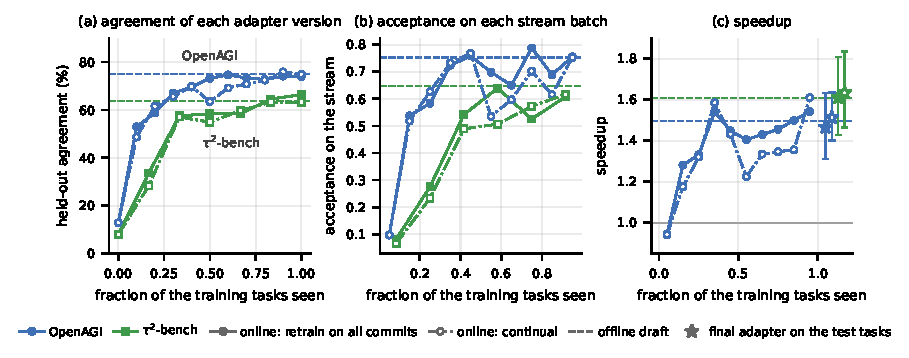
\includegraphics[width=\linewidth]{figures/fig_online_stream.pdf}
\caption{\textbf{Online training of the draft.} The draft is trained online, from the commits of the running
speculative system: the untrained 0.6B draft starts the system on the training tasks, and after every
batch a new adapter replaces the previous one in the draft server without a restart. Colour marks the
benchmark. Solid lines retrain the adapter on all commits so far; dash-dot lines with hollow markers
continue the previous adapter (continual). (a) Offline agreement of each adapter version on the held-out
contexts. (b) Acceptance on each batch of the stream. (c) Speedup on each OpenAGI batch and, as stars with
bootstrap intervals, the final adapters on the test tasks. Dashed: the offline drafts
(Tables~\ref{tab:offline} and~\ref{tab:four}); grey line: no speedup.}
\label{fig:online_stream}
\end{figure}

Figures~\ref{fig:online} and~\ref{fig:online_stream} show the result. On OpenAGI the draft agrees on 53\% of the held-out contexts
after 25 tasks, 67\% after 75, and 74.0\% after all 250 (offline draft: 75.0\%). The speedup on the stream
follows: 0.95\xx{} on the first batch with the untrained draft, 1.28\xx{} on the second, and 1.4--1.5\xx{}
from the fourth batch on. The final adapter gives 1.47\xx{} [1.31, 1.63] on the test tasks, against
1.51\xx{} [1.38, 1.64] for the offline draft under the same serving configuration. On $\tau^2$-bench, with tools executed, agreement on the validation
contexts goes from 8.0\% to 66.4\% (offline draft: 63.7\%), acceptance on the stream reaches the offline
draft's level after 30 tasks, and the final adapter gives 1.61\xx{} [1.43, 1.81] on the test tasks, the same
as the offline draft's 1.61\xx{} [1.44, 1.79]. The buffer ends with 1,079 pairs on OpenAGI, against 1,090 in
the offline training set, because the committed trajectories are the target's own.

Retraining on the whole buffer costs more with every batch (27 to 73 seconds per version on OpenAGI, 3 to
18 minutes on $\tau^2$-bench). A continual variant instead continues the previous adapter on the new batch plus an
equal-size sample of earlier pairs, for two epochs, at a fixed 22 seconds per update on OpenAGI. It reaches
the same endpoint (74.9\% agreement, 1.51\xx{} [1.40, 1.64] on the test tasks) but dips once on the way
(63.5\% and 1.22\xx{} at the fifth batch) before recovering. On $\tau^2$-bench it takes 3 to 6 minutes per update
instead of 3 to 18, ends at 63.3\% agreement (offline draft: 63.7\%), and gives 1.63\xx{} [1.46, 1.83] on the
test tasks. Appendix~\ref{app:online} gives the details.

\section{Additional limitations}
\label{app:limitations}
The speedups are 1.2--1.6\xx{}, and the framework of Sec.~\ref{sec:model} explains why they are not larger on
these benchmarks: tasks are short (4--14 steps), BFCL's user turns cut segments to 2.6 steps, and the
round cost $\beta$ of the trained drafts is 1.1--1.3. We evaluate two
target families (Qwen3-32B and Gemma-4-31B) on one GPU class, and our tools run against local simulated backends. With added tool latency the speedup
falls, to 1.20\xx{} on $\tau^2$-bench and 1.02\xx{} on BFCL at 5\,s per tool step (Table~\ref{tab:tool}), because the
draft's proposals execute their tools while proposing; with slow tools the tool-overlap
mechanisms of \citet{stc,swm,aospec} would matter more than ours. Every action LEAP executes is
target-authored, but the trajectories are not those of a target-only run: speculation changes which requests the
engine decodes together, and on the tool benchmarks, whose steps reason for 10--12\,s, most speculative
trajectories take a different decision at some step (App.~\ref{app:success}; two $\tau^2$-bench tasks even ran to
the token budget in the speculative arm only). Task success shows no systematic change. Proposing and verifying do not overlap, so the draft's cost is paid in full; a draft that ran ahead of the
target would hide that term, which Eq.~\ref{eq:S} without the draft term puts at 1.47$\to$1.72\xx{} on OpenAGI
and 1.46$\to$1.66\xx{} on TaskBench and at a few hundredths on the tool benchmarks. Verification issues up to
$k{+}1$ target generations per round (1.16\xx{} the sequential completion tokens on $\tau^2$-bench), so the
method trades compute for latency. Test sets are 40--63 tasks; task-level bootstrap intervals of the pooled
ratio are 0.15--0.30 wide (Table~\ref{tab:four}), so differences of a few
hundredths between configurations are not resolved by these runs. The online experiment of
Sec.~\ref{sec:online} makes one pass over each benchmark's training split; retraining on the whole buffer
costs more with every batch, and the continual variant that fixes this cost dipped once on OpenAGI before recovering,
which we have not studied further.
